\documentclass[12pt,a4paper]{article}
\usepackage{tpl}
\dbegin{Кружок для 7 класса, начинающие, школа 179}{Решения занятия №15}

\z У всех глупых марсиан по 3 руки, а некоторые трёхрукие марсиане пьют кефир. Можно ли утверждать, что некоторые глупые марсиане пьют кефир?

\s Нет, нельзя. Может быть, что половина трёхруких марсиан глупые и не пьют кефир, а остальные --- умные и пьют.\QEDA\\

\z Оля и Аня живут в одном доме и выходят в школу вместе. Каждый шаг Оли на $10\%$ длиннее Аниного, но Оля делает в минуту на $10\%$ меньше шагов, чем Аня. Кто раньше придёт в школу?

\s Олин шаг в $\frac{11}{10}$ раз длиннее, но в минуту она делает $\frac{9}{10}$ от количества шагов Ани. Значит, за минуту она проходит $\frac{99}{100}$ от расстояния, проходимого Аней. Аня идёт быстрее и придёт раньше.\QEDA\\

\n Чему равна последняя цифра числа $6^{2019}$?
\p $9^{2019}$?
\p $17^{2019}$?
\p $22^{2019}$?

\s Будем рассматривать цикл, по которому изменяется остаток $k^n$ по модулю 10 при изменении $n$ (это и будет его последняя цифра).
\setcounter{sprobs}{0}

\p $6\to6$, ответ --- 6.

\p $9\to1\to9$, ответ --- 9.

\p $7\to9\to3\to1\to7$, ответ --- 3.

\p $2\to4\to8\to6\to2$, ответ --- 8.\QEDA\\

\z В трёх коробках лежат шары: в одной --- два белых, в другой --- два чёрных, в третьей --- белый и чёрный. На коробках наклеены этикетки ББ, ЧЧ и БЧ так, что содержимое каждой коробки не соответствует этикетке. Как, вынув один шар, узнать, в какой коробке что лежит?

\s Вынем шар из коробки БЧ. Не умаляя общности, он чёрный, и там было два чёрных шара. Значит, в ББ белый и чёрный, а в ЧЧ --- два белых.\QEDA\\

\z На столе лежат четыре яблока весом 200г, 300г, 400г и 450г. Карлсон, а затем Малыш берут по яблоку и одновременно начинают есть их с одинаковой скоростью. Доевший берет следующее яблоко, каждый хочет съесть как можно больше. Какое яблоко выбрать Карлсону вначале?

\s Карлсон берёт яблоко в 300 граммов. К тому моменту, как он его доест, яблоко либо в 400 граммов, либо в 450 граммов будет свободно. С ним Карлсон набирает больше половины. Ответ находится перебором яблок.\QEDA\\

\z Леспромхоз решил вырубить сосновый лес, но экологи запротестовали. Тогда директор леспромхоза всех успокоил, сказав: <<В лесу $99\%$ сосен. Мы будем рубить только сосны. После порубки сосны будут составлять $98\%$ всех деревьев>>. Какую часть леса вырубит леспромхоз?

\s Изначально деревьев было в 100 раз больше, чем не-сосен, а стало в 50 раз больше, чем не-сосен. При этом количество не-сосен не изменилось. Ответ: половину леса.\QEDA\\

\z Петя заметил, что у всех его 25 одноклассников различное число друзей в этом классе. Сколько друзей в классе у Пети? (Найдите все решения).

\s Рассмотрим Васю --- одноклассника Пети, у которого больше всего друзей, и Колю --- одноклассника, у которого меньше всего друзей. Заметим, что либо у Коли 0 друзей, либо у Васи все ученики класса (кроме него самого) --- друзья. В обоих случаях Вася дружит с Петей, а Коля нет. Уберём из класса Васю и Колю. Все количества друзей у одноклассников Пети снова различны, у Пети теперь на 1 друга меньше, в классе на 2 человека меньше. Так можно сделать 12 раз, после чего останется Петя и ещё один человек. Они либо дружат, либо нет, причём оба варианта возможны. Ответ: 12 или 13.\QEDA\\

\newpage
\z Из листа клетчатой бумаги размером $11\times11$ клеток вырезали по клеткам 15 квадратиков $2\times2$ клетки. Докажите, что можно вырезать еще один такой квадратик.

\s См. рисунок. Каждый квадрат пересекается ровно с одним нарисованным.\QEDA\\

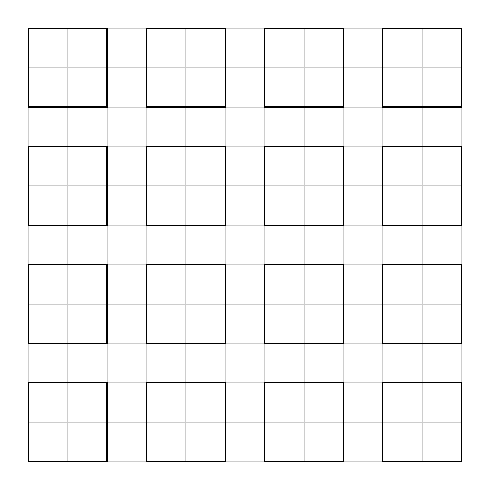
\begin{tikzpicture}
	\draw[step=0.5,very thin,black!20] (0,0) grid (5.5,5.5);
	\path[draw] (0,0)--(1,0)--(1,1)--(0,1)--cycle;
	\path[draw] (0,1.5)--(1,1.5)--(1,2.5)--(0,2.5)--cycle;
	\path[draw] (0,3)--(1,3)--(1,4)--(0,4)--cycle;
	\path[draw] (0,4.5)--(1,4.5)--(1,5.5)--(0,5.5)--cycle;
	\path[draw] (1.5,0)--(2.5,0)--(2.5,1)--(1.5,1)--cycle;
	\path[draw] (1.5,1.5)--(2.5,1.5)--(2.5,2.5)--(1.5,2.5)--cycle;
	\path[draw] (1.5,3)--(2.5,3)--(2.5,4)--(1.5,4)--cycle;
	\path[draw] (1.5,4.5)--(2.5,4.5)--(2.5,5.5)--(1.5,5.5)--cycle;
	\path[draw] (3,0)--(4,0)--(4,1)--(3,1)--cycle;
	\path[draw] (3,1.5)--(4,1.5)--(4,2.5)--(3,2.5)--cycle;
	\path[draw] (3,3)--(4,3)--(4,4)--(3,4)--cycle;
	\path[draw] (3,4.5)--(4,4.5)--(4,5.5)--(3,5.5)--cycle;
	\path[draw] (4.5,0)--(5.5,0)--(5.5,1)--(4.5,1)--cycle;
	\path[draw] (4.5,1.5)--(5.5,1.5)--(5.5,2.5)--(4.5,2.5)--cycle;
	\path[draw] (4.5,3)--(5.5,3)--(5.5,4)--(4.5,4)--cycle;
	\path[draw] (4.5,4.5)--(5.5,4.5)--(5.5,5.5)--(4.5,5.5)--cycle;
\end{tikzpicture}

\n Двое играют в такую игру: имеется куча из 21 камня, ходят по очереди, за ход игрок забирает из кучи 1 или 3 камня. Выигрывает тот, кто возьмёт последний камень. Кто выиграет при правильной игре и как ему играть?

\s Вне зависимости от того, как ходят игроки, игра продлится нечётное количество ходов, так как сумма чётного количества единиц и троек чётна. Значит, выиграет первый.\QEDA

\p То же, но можно брать 1, 2 или 4 камня.

\s Докажем, что первый проигрывает тогда и только тогда, когда текущее количество камней делится на 3. Действительно, если оно не делится, то можно вычесть 1 или 2 так, чтобы оно разделилось, а если делится, то в любом случае после хода делиться не будет. Кроме того, если камней 0, то проигрывает первый. Сейчас камней 21, это число делится на 3, значит, выигрывает второй.\QEDA

\p То же, но можно брать 1, 3 или 4 камня.

\s Докажем, что первый проигрывает тогда и только тогда, когда текущее количество камней даёт остаток 0 или 2 при делении на 7.\footnote{Это можно понять так. Если в кучке 0 камней, выигрывает второй, если 1, 3 или 4 камня, выигрывает первый, если 2 --- второй, если 5 или 6 --- первый, если 7 --- второй, и т.п.} Действительно, из всех остальных остатков можно перейти в один из этих двух; из этих двух можно перейти только в другой остаток; количество камней в финальной позиции (в которой проигрывает тот, чей сейчас ход) имеет остаток 0. Сейчас оно 0, значит, выигрывает второй.\QEDA\\

\end{document}
